\documentclass[10pt,twocolumn,letterpaper]{article}

\usepackage[T1]{fontenc}
\usepackage[utf8]{inputenc}
\usepackage{newtxtext,newtxmath}
\usepackage[letterpaper,top=0.52in,bottom=0.55in,left=0.62in,right=0.62in,columnsep=0.24in]{geometry}
\usepackage{graphicx}
\usepackage{amsmath}
\usepackage{booktabs}
\usepackage{array}
\usepackage{microtype}
\usepackage{caption}
\usepackage[hidelinks]{hyperref}
\usepackage{url}

\setlength{\parindent}{1em}
\setlength{\parskip}{0pt}
\setlength{\textfloatsep}{5pt plus 1pt minus 1pt}
\setlength{\floatsep}{5pt plus 1pt minus 1pt}
\setlength{\intextsep}{5pt plus 1pt minus 1pt}
\captionsetup{font=small,labelfont=bf,skip=2pt}
\renewcommand{\arraystretch}{1.08}
\newcommand{\submissioncommit}{\texttt{{{COMMIT_HASH}}}}

\begin{document}

\twocolumn[
\begin{center}
{\LARGE\bfseries Bagging, Boosting and Measured Bias--Variance\\
for Olivetti Face Recognition\par}
\vspace{5pt}
{\large\bfseries Dishant Kaushik} \quad $|$ \quad Roll number: M24MA2003\\
Email: \href{mailto:m24ma2003@iitj.ac.in}{m24ma2003@iitj.ac.in}\\
Repository: \url{https://github.com/dishant1901-prog/machine-learning-assignment-2}\\
Submission commit: \submissioncommit
\end{center}

\begin{minipage}{0.96\textwidth}
\begin{center}\textbf{Abstract}\end{center}
This study compares a decision-tree baseline with scratch implementations of bootstrap aggregation and multiclass SAMME on the 40-class Olivetti face task. All choices are made on one fixed validation split before test evaluation. Bagging 200 unrestricted trees gives 87.50\% clean-test accuracy and remains strongest after a centred $16\times16$ region is removed (70.00\%). The selected depth-4, 100-round SAMME model is faster but reaches 52.50\% on the clean test. Thirty identity-stratified training resamples show why: bagging has variance 0.02062, compared with 0.64272 for a single tree, whereas boosting has the lowest variance (0.01587) but the highest squared bias (0.88015). Thus stability alone does not determine recognition accuracy.

\vspace{4pt}
\centering
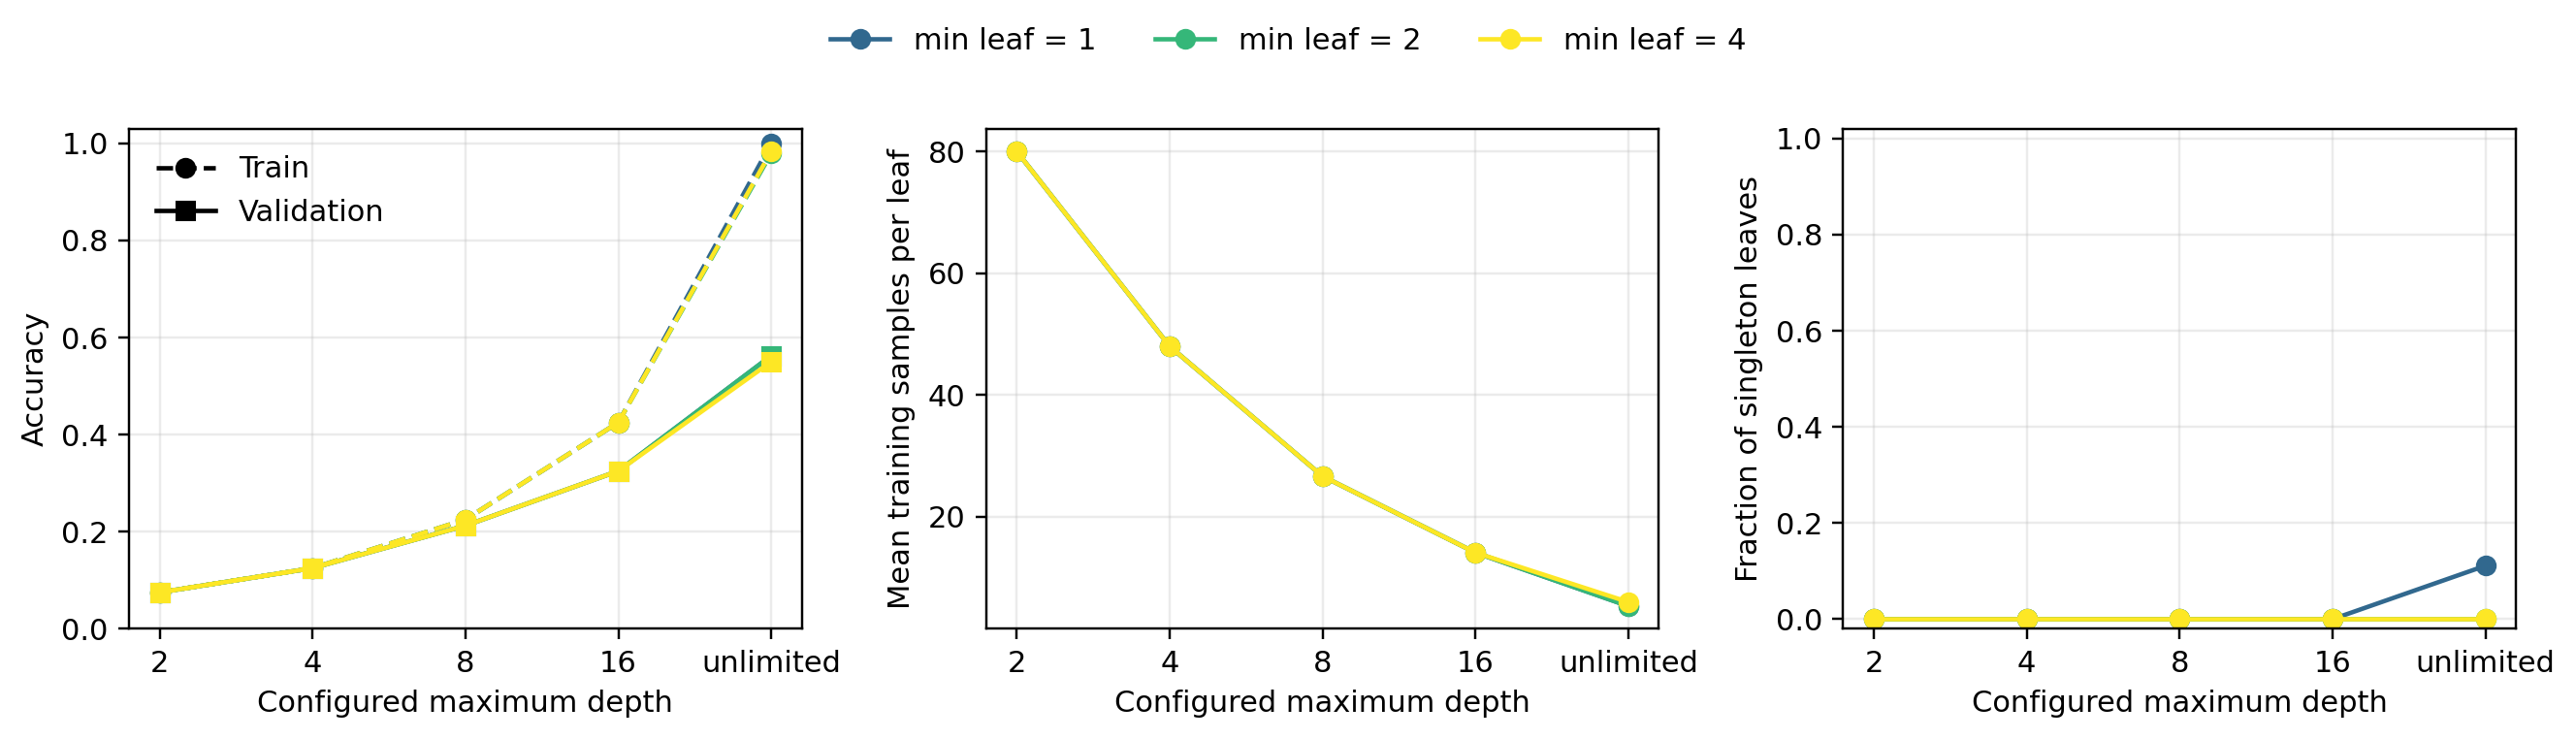
\includegraphics[width=0.92\textwidth]{../question_1/outputs/figures/q1a_depth_diagnostics.png}
\captionof{figure}{Complete Q1 tree grid. Depth improves fit and validation accuracy, but also produces smaller, less populated leaves.}
\end{minipage}
\vspace{5pt}
]

\section{Experimental protocol}
The Olivetti data contain ten $64\times64$ grayscale images for each of 40 identities~\cite{samaria1994}. I used the 4096 raw pixels directly. The numeric part of the roll number gives seed 242003. Within every identity I drew a deterministic 6/2/2 train/validation/test split, giving 240, 80 and 80 images. The saved split digest begins \texttt{5f1c58f7}.

Hyperparameters were selected only by clean validation accuracy. The clean and masked test sets were not used for selection. The masked set is a copy of the fixed test set with rows and columns 24--39 set to zero. Training always uses clean faces.

I used scikit-learn only for individual \texttt{DecisionTreeClassifier} models~\cite{pedregosa2011}. Bootstrap sampling, hard voting, out-of-bag accounting and SAMME were implemented directly. Smaller bagging ensembles are prefixes of the same 200-tree run, which keeps their comparisons paired.

\section{Q1: Tree and bagging}
\subsection{Single-tree baseline}
The grid covered maximum depths 2, 4, 8, 16 and unrestricted, with minimum leaf sizes 1, 2 and 4. Unrestricted trees with leaf sizes 1 and 2 tied at 56.25\% validation accuracy. The declared simplicity tie-break selected leaf size 2, eliminating singleton leaves without reducing validation accuracy.

\begin{table}[h]
\centering\scriptsize
\resizebox{\columnwidth}{!}{%
\begin{tabular}{lrrrrrr}
\toprule
Model & Train & Val. & Test & Leaves & Mean/leaf & Singleton \\
\midrule
Tree (unrestricted, leaf 2) & 97.92 & 56.25 & 57.50 & 45 & 5.33 & 0\% \\
\bottomrule
\end{tabular}}
\end{table}

For leaf size 2, increasing depth from 2 to unrestricted raises the leaf count from 3 to 45 and lowers mean occupancy from 80.00 to 5.33. Training accuracy rises from 7.50\% to 97.92\%, while validation reaches only 56.25\%. This widening gap is the measured cost of increasingly specialised partitions.

\subsection{Bagging from scratch}
Each tree receives 240 bootstrap draws and uses the frozen tree setting. Aggregation follows Breiman's plurality-vote construction~\cite{breiman1996}.

\begin{table}[h]
\centering\scriptsize
\begin{tabular}{rrrrr}
\toprule
$B$ & Train & Val. & Test & Distinct \\
\midrule
1   & 72.08  & 32.50 & 35.00 & 151.00 \\
5   & 95.42  & 50.00 & 62.50 & 153.40 \\
10  & 99.17  & 70.00 & 68.75 & 151.50 \\
25  & 100.00 & 76.25 & 76.25 & 151.16 \\
50  & 100.00 & 82.50 & 81.25 & 150.76 \\
100 & 100.00 & 81.25 & 83.75 & 151.05 \\
200 & 100.00 & \textbf{86.25} & 87.50 & 151.85 \\
\bottomrule
\end{tabular}
\end{table}

For sample size $n$, the expected number of represented cases is
$n[1-(1-1/n)^n]$. At $n=240$ this is 151.893 (63.289\%), close to $1-e^{-1}$. The measured 200-tree mean is 151.85 (63.271\%). Validation accuracy is not monotone---$B=50$ slightly exceeds $B=100$---but $B=200$ is best and was frozen before its test result was used.

\clearpage
\subsection{OOB accuracy, disagreement and margin}
\begin{figure*}[t]
\centering
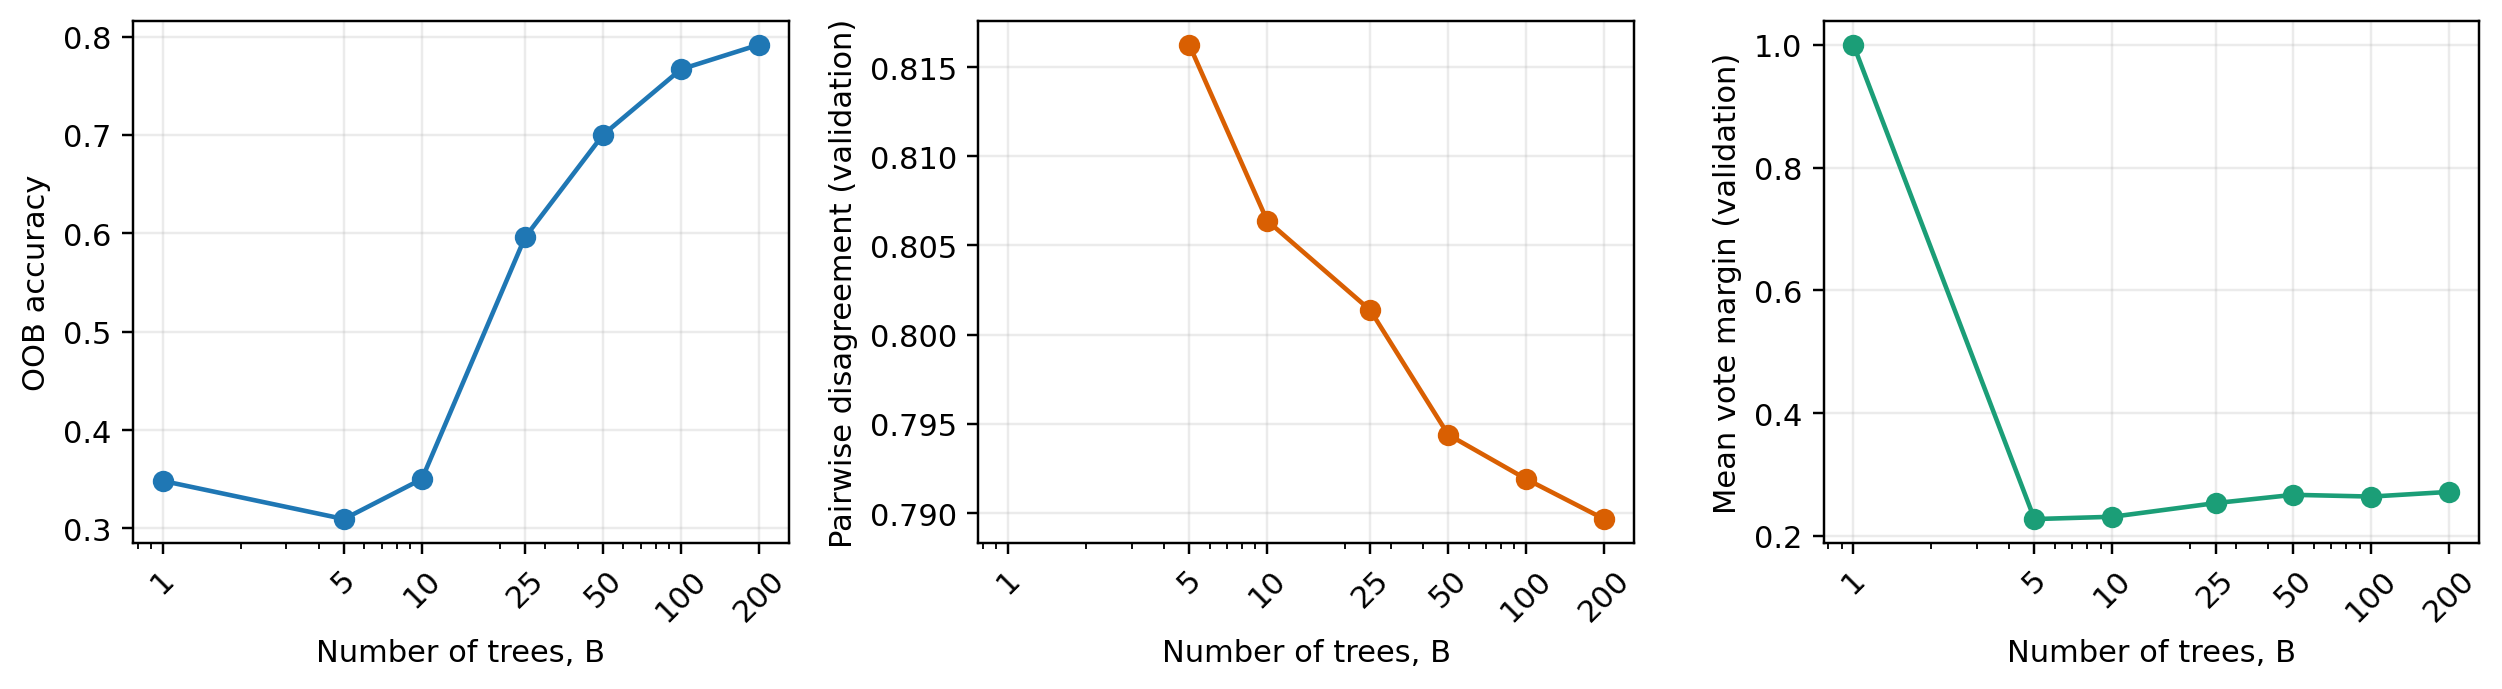
\includegraphics[width=0.94\textwidth]{../question_1/outputs/figures/q1c_oob_disagreement_margin.png}
\caption{OOB accuracy and coverage, validation-set pairwise disagreement, and validation vote margin. $B=1$ disagreement is undefined; its unit margin is a one-vote artifact.}
\end{figure*}

\begin{table}[h]
\centering\scriptsize
\begin{tabular}{rrrrr}
\toprule
$B$ & OOB acc. & Coverage & Disagree. & Margin \\
\midrule
1   & 34.83 & 37.08  & --     & 1.0000 \\
5   & 30.95 & 87.50  & 0.8163 & 0.2275 \\
10  & 35.02 & 98.75  & 0.8064 & 0.2313 \\
25  & 59.58 & 100.00 & 0.8014 & 0.2535 \\
50  & 70.00 & 100.00 & 0.7944 & 0.2670 \\
100 & 76.67 & 100.00 & 0.7919 & 0.2641 \\
200 & 79.17 & 100.00 & 0.7897 & 0.2718 \\
\bottomrule
\end{tabular}
\end{table}

OOB coverage is only 37.08\% at $B=1$ and reaches 100\% by $B=25$. Thereafter OOB accuracy rises from 59.58\% to 79.17\%. The validation margin generally increases, but disagreement falls slightly from 0.8163 at $B=5$ to 0.7897 at $B=200$. More trees do not create increasing diversity; they average many already diverse, noisy decisions until the leading class becomes more stable.

\subsection{Clean and masked faces}
\begin{table}[h]
\centering\scriptsize
\begin{tabular}{llrr}
\toprule
Model & Set & Accuracy & Confidence \\
\midrule
Tree & Clean & 57.50 & 0.9813 \\
Tree & Masked & 33.75 & 1.0000 \\
Bagging (200) & Clean & 87.50 & 0.4079 \\
Bagging (200) & Masked & 70.00 & 0.2974 \\
\bottomrule
\end{tabular}
\end{table}

Masking costs the tree 23.75 percentage points and bagging 17.50. The tree's leaf-probability confidence rises to 1.0 while its accuracy collapses: masked images are being routed into pure leaves, not recognised more reliably. Bagging confidence, defined as the winning vote fraction, falls as expected.

For identities 0 and 1 (indices 6 and 10), the tree predicts 15 and 16, while 65 and 74 bagged trees recover the correct classes. These are unstable partition errors. The shared mistakes differ. Identity 4 (index 41) is nearly tied between wrong class 37 (58 votes) and true class 4 (53); identity 12 (index 127) receives only eight correct votes amid a diffuse set of alternatives. Aggregation can remove unstable errors, but not errors shared by most base models.

\begin{figure}[h]
\centering
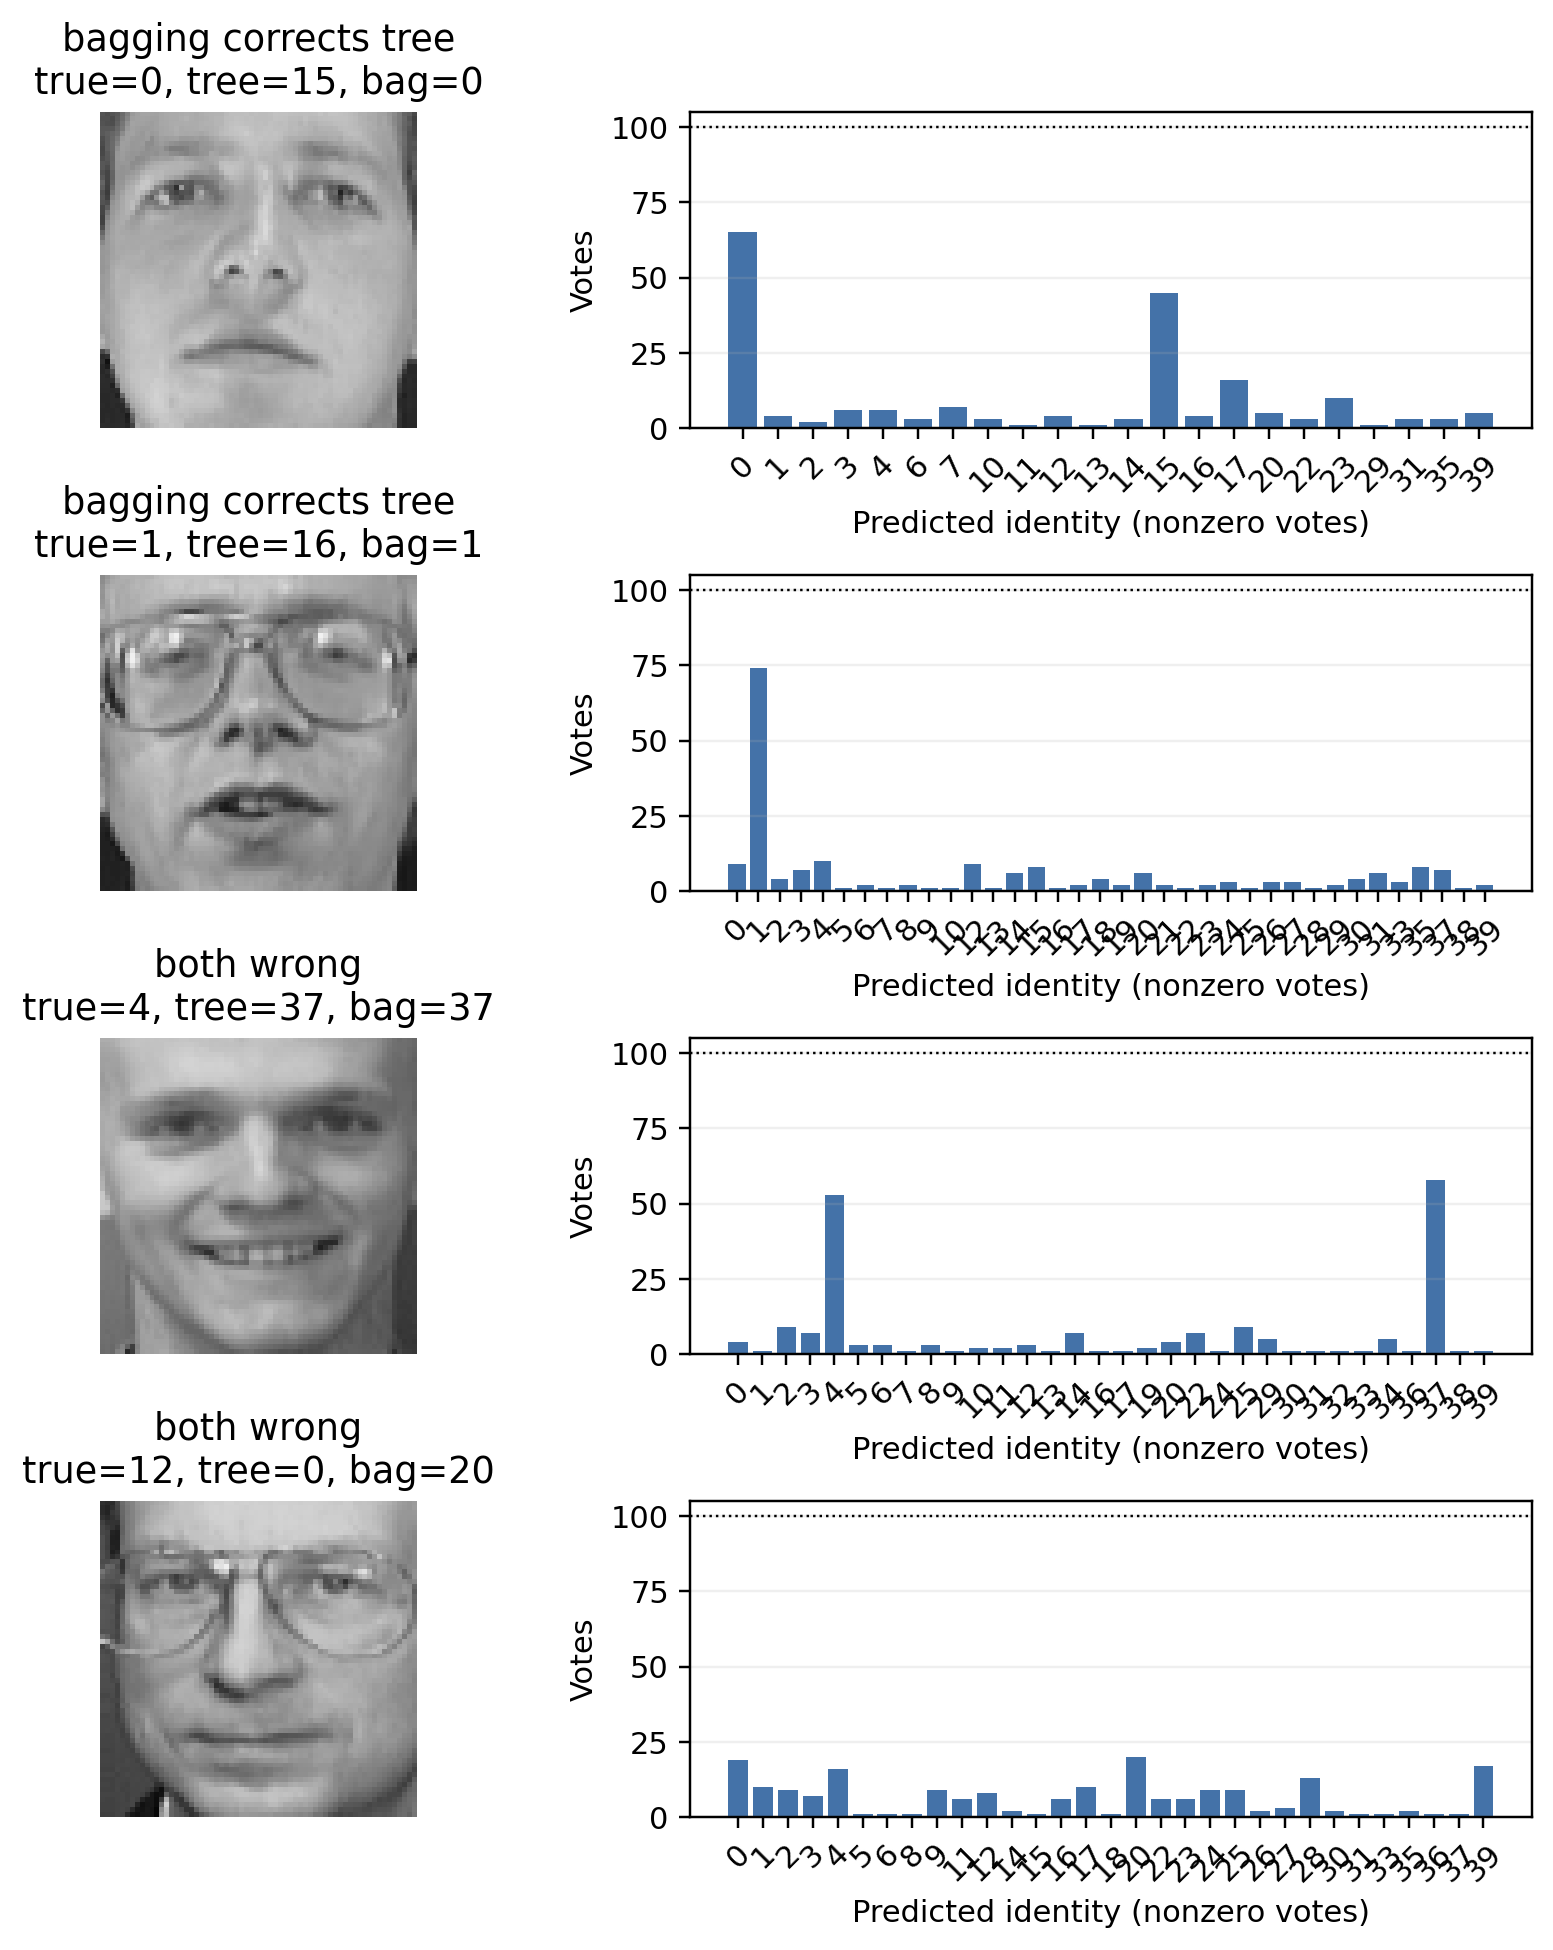
\includegraphics[width=0.93\columnwidth]{../question_1/outputs/figures/q1d_case_evidence.png}
\caption{Two clean faces where bagging corrects the tree and two where both fail. Each panel gives the true label, tree prediction and all nonzero bagging votes.}
\end{figure}

\clearpage
\section{Q2: Multiclass SAMME}
\subsection{One complete three-class round}
My scratch implementation follows the SAMME weighted error and class-score construction~\cite{zhu2009}:
\begin{align}
\alpha_t &= \log\!\left(\frac{1-\epsilon_t}{\epsilon_t}\right)+\log(K-1),\\
S_k(x) &= \sum_t \alpha_t\,\mathbf{1}[h_t(x)=k].
\end{align}
The toy problem has nine one-dimensional samples: three consecutive examples from each of classes 0, 1 and 2. A depth-1 tree predicts $[0,0,0,1,1,1,1,1,1]$. With initial weights $1/9$, the last three samples are wrong, so $\epsilon=1/3$ and $\alpha=\log(4)=1.386294$. The update is $w_i\leftarrow w_i\exp(\alpha\mathbf{1}[\mathrm{wrong}])$.

\begin{table}[h]
\centering\scriptsize
\resizebox{\columnwidth}{!}{%
\begin{tabular}{lrrrrrr}
\toprule
Samples & True & Pred. & Initial & Wrong & Unnorm. & Final \\
\midrule
0--2 & 0 & 0 & $1/9$ & No  & $1/9$ & $1/18$ \\
3--5 & 1 & 1 & $1/9$ & No  & $1/9$ & $1/18$ \\
6--8 & 2 & 1 & $1/9$ & Yes & $4/9$ & $2/9$ \\
\bottomrule
\end{tabular}}
\end{table}

The unnormalised weights sum to 2. The face code calls this same update. A learner is accepted only when $\epsilon<1-1/K$; an invalid learner is logged and training stops. Zero error uses a numerical floor for finite $\alpha$ and then stops. Tests cover both cases, and no learner was rejected in the official run.

\subsection{Validation selection}
The matrix gives validation accuracy (\%) for each depth/round pair. Selection used no test values.

\begin{table}[h]
\centering\scriptsize
\begin{tabular}{lrrrr}
\toprule
Depth $\backslash$ rounds & 10 & 25 & 50 & 100 \\
\midrule
1 & 5.00 & 10.00 & 10.00 & 11.25 \\
2 & 7.50 & 8.75 & 16.25 & 20.00 \\
3 & 16.25 & 25.00 & 22.50 & 32.50 \\
4 & 17.50 & 26.25 & 43.75 & \textbf{51.25} \\
\bottomrule
\end{tabular}
\end{table}

Depth 4 with 100 rounds was best and therefore frozen. It reaches 100\% training accuracy but only 51.25\% validation accuracy. By contrast, 100 depth-1 learners reach 15.83\% training accuracy, so very shallow partitions underfit this 40-class problem.

\begin{figure}[h]
\centering
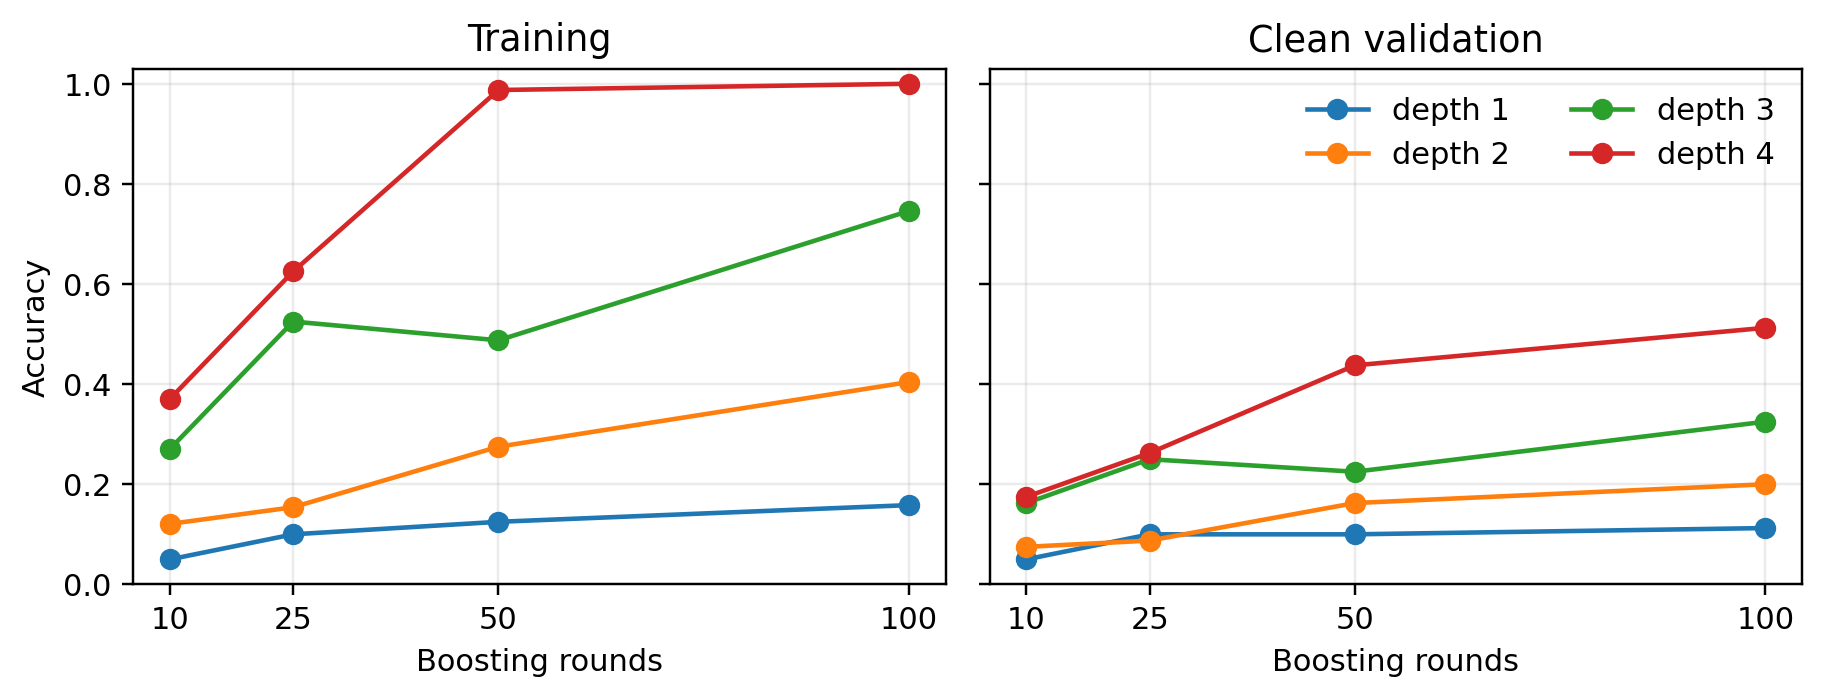
\includegraphics[width=\columnwidth]{../question_2/outputs/figures/q2b_validation_grid.png}
\caption{Training and validation accuracy over the complete boosting grid.}
\end{figure}

\begin{figure}[h]
\centering
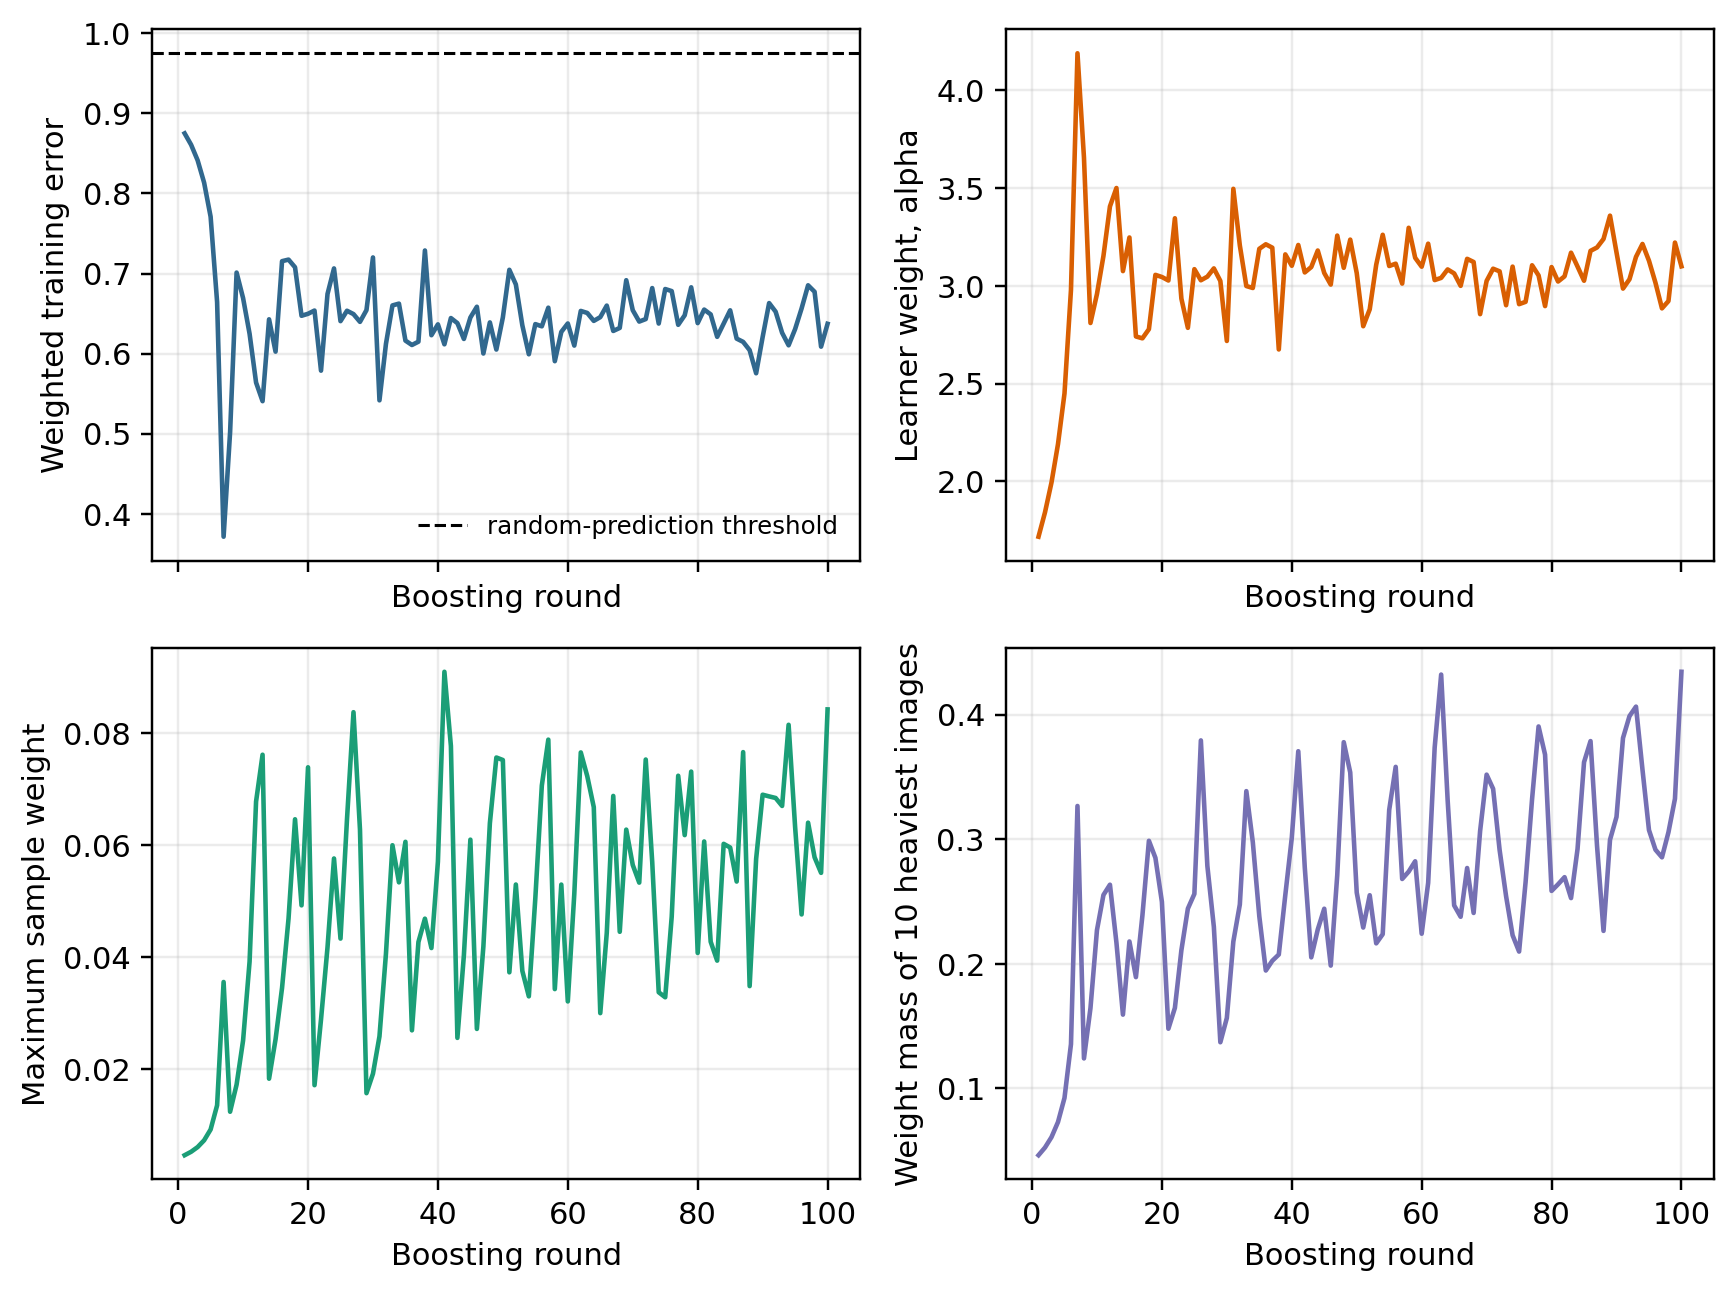
\includegraphics[width=0.94\columnwidth]{../question_2/outputs/figures/q2b_selected_round_diagnostics.png}
\caption{Per-round weighted error, learner weight, largest sample weight and total mass of the ten heaviest samples.}
\end{figure}

Across the selected run, weighted errors range from 0.3714 to 0.8750, always below the $39/40$ random threshold. Learner weights range from 1.7177 to 4.1897. The maximum individual weight reaches 0.0910 at round 41, and the ten heaviest faces carry 0.4344 of the mass at round 100.

\clearpage
\subsection{Bagging versus boosting}
\begin{figure*}[t]
\centering
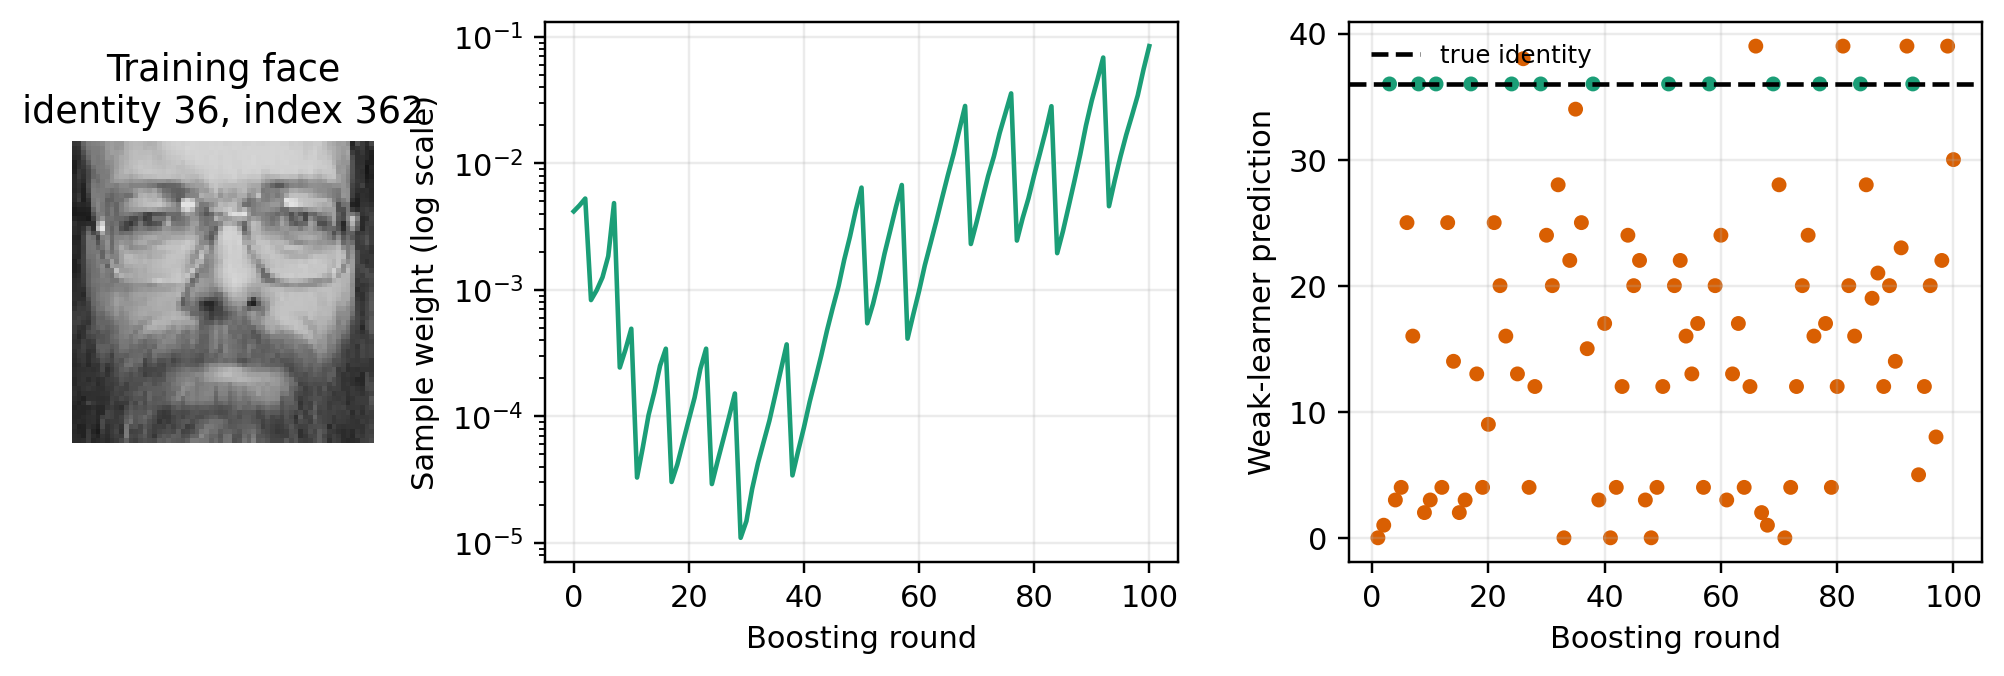
\includegraphics[width=0.92\textwidth]{../question_2/outputs/figures/q2c_heaviest_training_face.png}
\caption{Identity 36, dataset index 362, receives the largest final SAMME weight. The plot relates its prediction history to repeated changes in sample weight.}
\end{figure*}

\begin{table}[h]
\centering\scriptsize
\resizebox{\columnwidth}{!}{%
\begin{tabular}{rlrrrr}
\toprule
Learners & Model & Train & Val. & Test & Fit time (s) \\
\midrule
25  & Bagging  & 100.00 & 76.25 & 76.25 & 23.04 \\
25  & Boosting & 62.50  & 26.25 & 26.25 & 7.12 \\
50  & Bagging  & 100.00 & 82.50 & 81.25 & 45.33 \\
50  & Boosting & 98.75  & 43.75 & 43.75 & 14.44 \\
100 & Bagging  & 100.00 & 81.25 & 83.75 & 90.93 \\
100 & Boosting & 100.00 & 51.25 & 52.50 & 28.80 \\
\bottomrule
\end{tabular}}
\end{table}

Times cover only base-learner fitting on the same machine. Boosting is about three times faster because its trees stop at depth 4, whereas bagging uses unrestricted trees. At 100 learners, however, bagging is 31.25 points more accurate on the clean test.

Index 362 is misclassified in 87 of 100 rounds and finishes with weight 0.08428. Mistakes in rounds 89--92 raise it from 0.01170 to 0.06846; a correct round-93 prediction lowers it to 0.00458, then seven more mistakes return it to 0.08428. The wrong labels vary, indicating that successive shallow partitions rarely isolate this face rather than confusing it with one fixed identity.

\subsection{Missing-region response}
\begin{table}[h]
\centering\scriptsize
\resizebox{\columnwidth}{!}{%
\begin{tabular}{lrrrr}
\toprule
Model & Clean acc. & Clean conf. & Masked acc. & Masked conf. \\
\midrule
Tree & 57.50 & 0.9813 & 33.75 & 1.0000 \\
Bagging & 87.50 & 0.4079 & 70.00 & 0.2974 \\
Boosting & 52.50 & 0.1207 & 53.75 & 0.1143 \\
\bottomrule
\end{tabular}}
\end{table}

Boosting gains one correct prediction after masking, but its mean winning vote falls. I treat the 1.25-point increase as split-specific label flips, not evidence that removing information helps.

\begin{figure}[h]
\centering
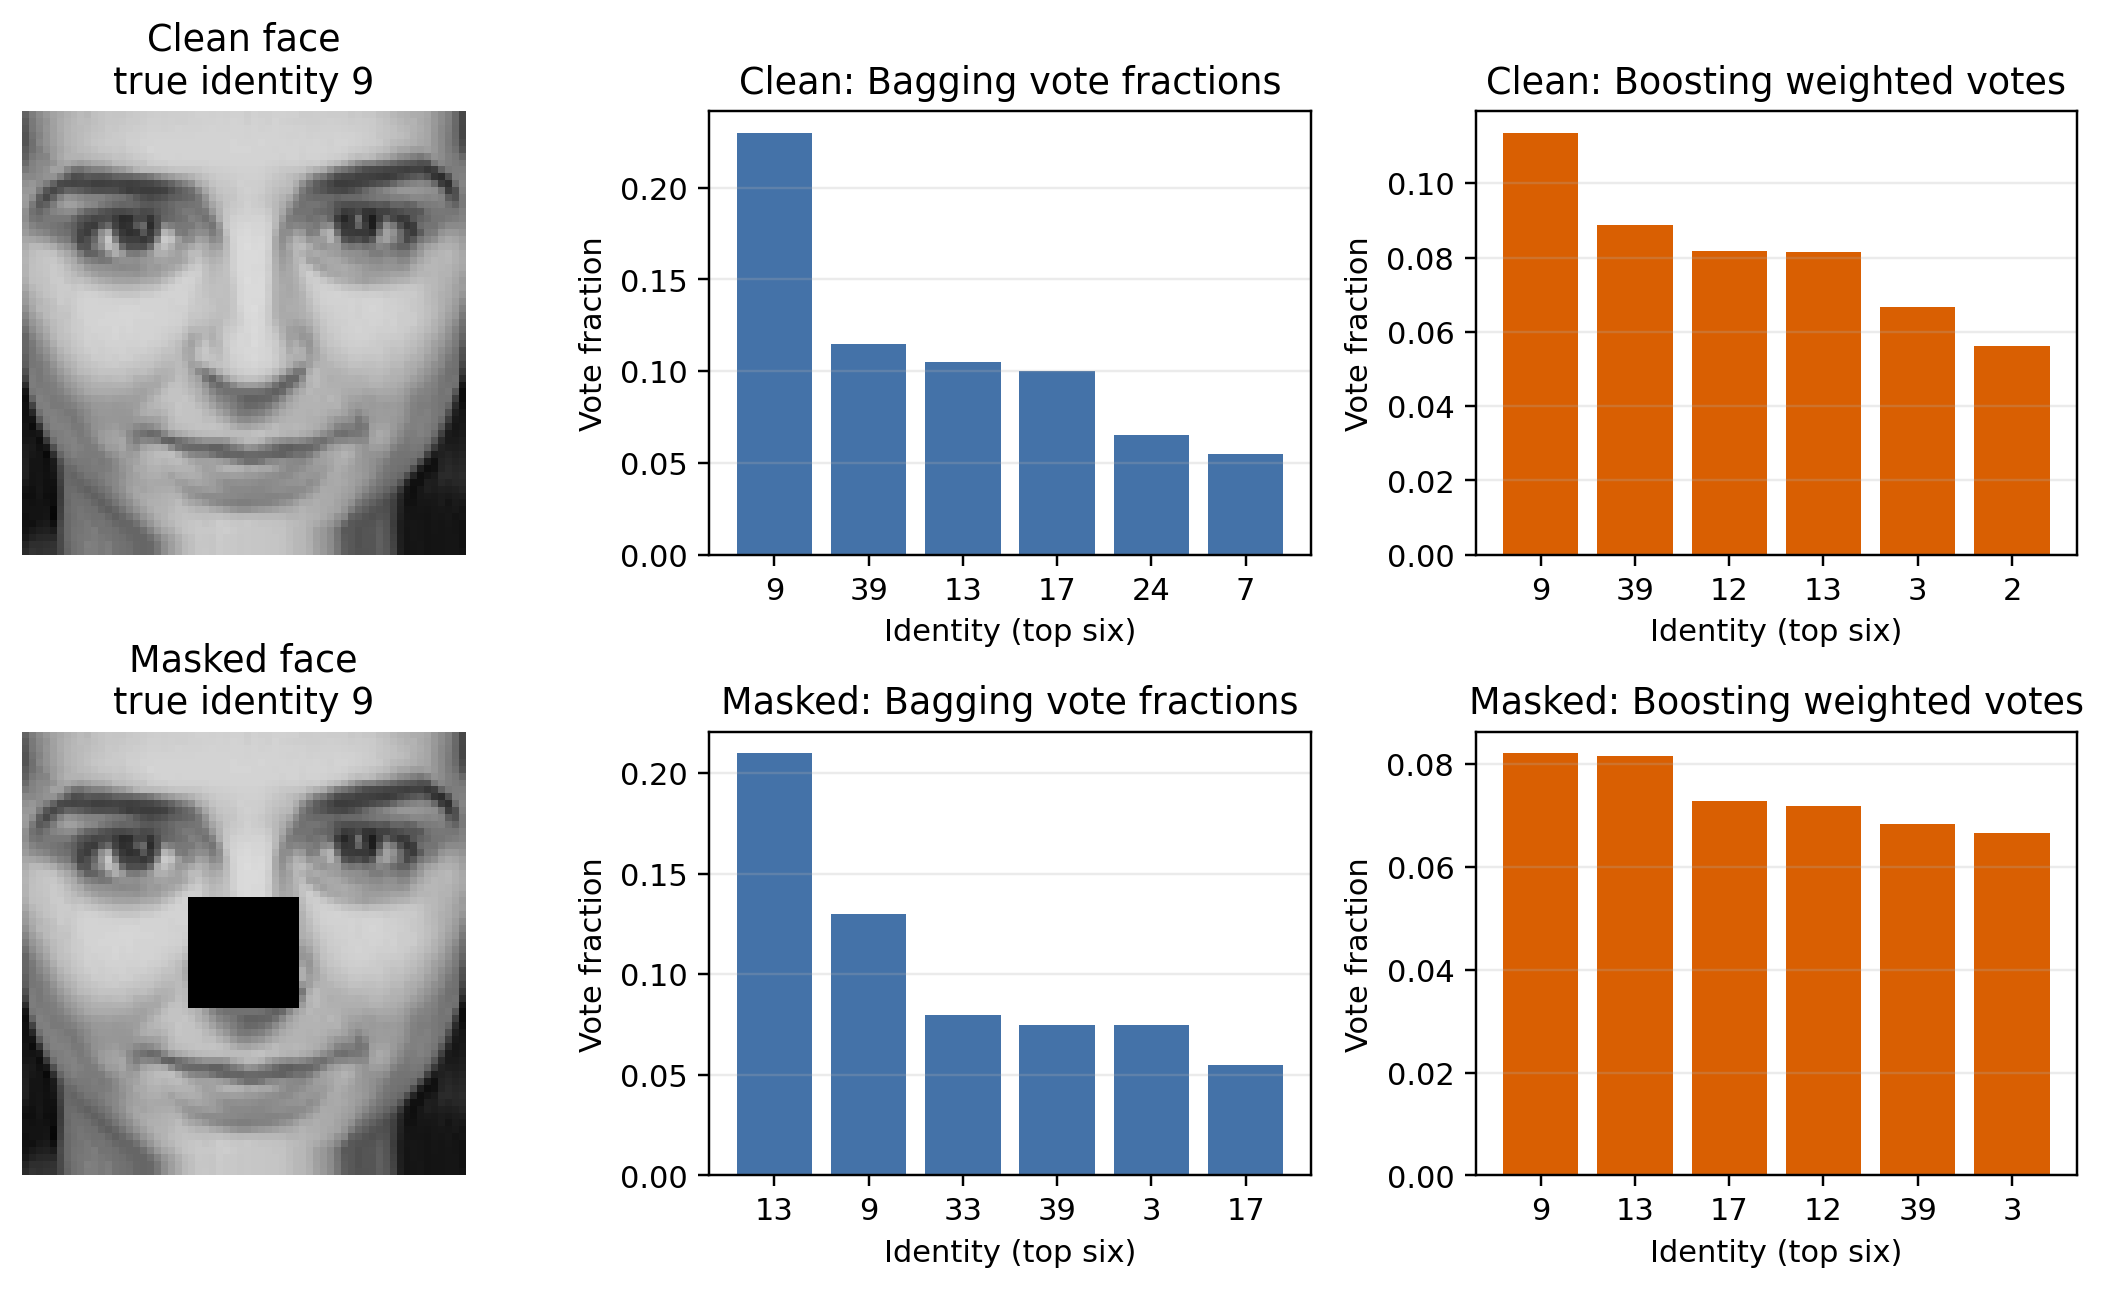
\includegraphics[width=0.96\columnwidth]{../question_2/outputs/figures/q2d_mask_response_case.png}
\caption{Identity 9, index 97, is correctly recognised by both clean models. Masking flips bagging but leaves boosting narrowly correct.}
\end{figure}

For this face, clean bagging gives identity 9 46/200 votes. After masking, 44.5\% of trees change prediction; disagreement rises from 0.9022 to 0.9132 and class 13 wins 42 votes against 26 for class 9. The winning margin falls from 0.115 to 0.080.

Only 15\% of boosting learners change label, carrying 15.64\% of total $\alpha$. Its correct class-9 weighted vote falls from 0.11363 to 0.08207, barely above class 13 at 0.08152---a margin of 0.00055. The sequentially trained depth-4 learners react more consistently for this face, but the near tie is fragile rather than confident.

\clearpage
\section{Q3: Bias and variance as measurements}
\subsection{Resampling and definitions}
I kept the 80 clean test faces fixed and generated 30 training sets. Within each identity, six draws with replacement came only from that identity's original six training faces. Every selected model was refitted without retuning.

For each test face I saved a 40-class vector: leaf probabilities for a tree, vote fractions for bagging, and normalised $\alpha$-weighted votes for boosting. For target one-hot vector $e_i$, prediction $p_r(x_i)$ and repetition mean $\bar p(x_i)$, I computed
\begin{align}
\mathrm{Bias}^2 &= \frac{1}{N}\sum_i \|\bar p(x_i)-e_i\|_2^2,\\
\mathrm{Variance} &= \frac{1}{NR}\sum_{i,r}\|p_r(x_i)-\bar p(x_i)\|_2^2.
\end{align}
Every vector was checked to have class order 0--39 and unit sum. Accuracy standard deviations use \texttt{ddof=1}; bias and variance use the population denominators above.

\subsection{Selected models over 30 refits}
\begin{table}[h]
\centering\scriptsize
\begin{tabular}{lrrrr}
\toprule
Model & Bias$^2$ & Variance & Mean acc. & SD \\
\midrule
Tree & 0.40394 & 0.64272 & 47.67 & 4.59 \\
Bagging (200) & 0.49887 & 0.02062 & \textbf{78.29} & 3.26 \\
Boosting (100) & 0.88015 & \textbf{0.01587} & 33.63 & 7.47 \\
\bottomrule
\end{tabular}
\end{table}

The unrestricted tree has the smallest bias but by far the largest variance. Bagging raises bias moderately and reduces variance by 96.79\% relative to the selected single tree when using 200 trees. Boosting is the most stable in the vector sense, yet its high bias leaves it least accurate on average. Bias and variance use the whole class vector, so neither is identical to classification error.

\begin{figure}[h]
\centering
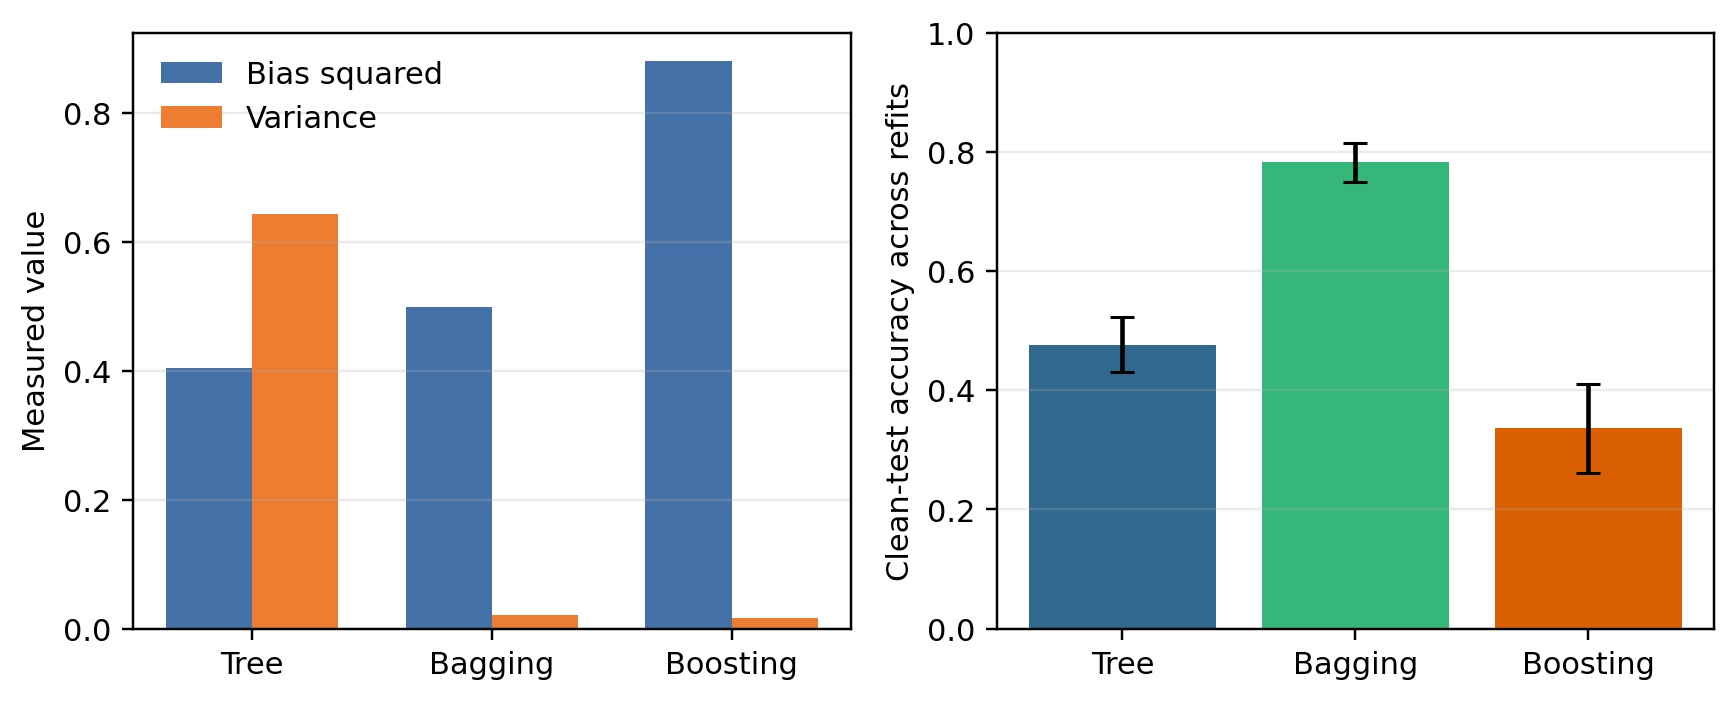
\includegraphics[width=\columnwidth]{../question_3/outputs/figures/q3a_selected_models.png}
\caption{Measured bias$^2$, variance and accuracy distribution for the three frozen models.}
\end{figure}

\subsection{Depth study}
Validation selected an unrestricted tree, so no finite limit can be deeper than the selected setting. I therefore predeclared depth 2 as shallow, depth 16 as a much deeper finite contrast, and retained the selected unrestricted model as the deepest setting. All trees use minimum leaf size 2; paired bagged ensembles use 100 trees.

\begin{table}[h]
\centering\scriptsize
\resizebox{\columnwidth}{!}{%
\begin{tabular}{llrrrr}
\toprule
Depth & Model & Bias$^2$ & Variance & Accuracy & Var. removed \\
\midrule
2 & Tree & 0.90476 & 0.04633 & 6.71 & -- \\
2 & Bagging & 0.92765 & 0.01063 & 14.21 & 77.05\% \\
16 & Tree & 0.63420 & 0.24113 & 29.17 & -- \\
16 & Bagging & 0.65462 & 0.01987 & 67.12 & 91.76\% \\
None & Tree & 0.40394 & 0.64272 & 47.67 & -- \\
None & Bagging & 0.49893 & 0.02450 & 77.12 & 96.19\% \\
\bottomrule
\end{tabular}}
\end{table}

Increasing depth lowers single-tree bias and sharply raises variance. Bagging removes 0.03570, 0.22126 and 0.61822 variance units at depths 2, 16 and unrestricted. The small accompanying increase in bias is outweighed by variance removal for the deeper settings.

\clearpage
\subsection{Does the deepest setting gain most?}
\begin{figure*}[t]
\centering
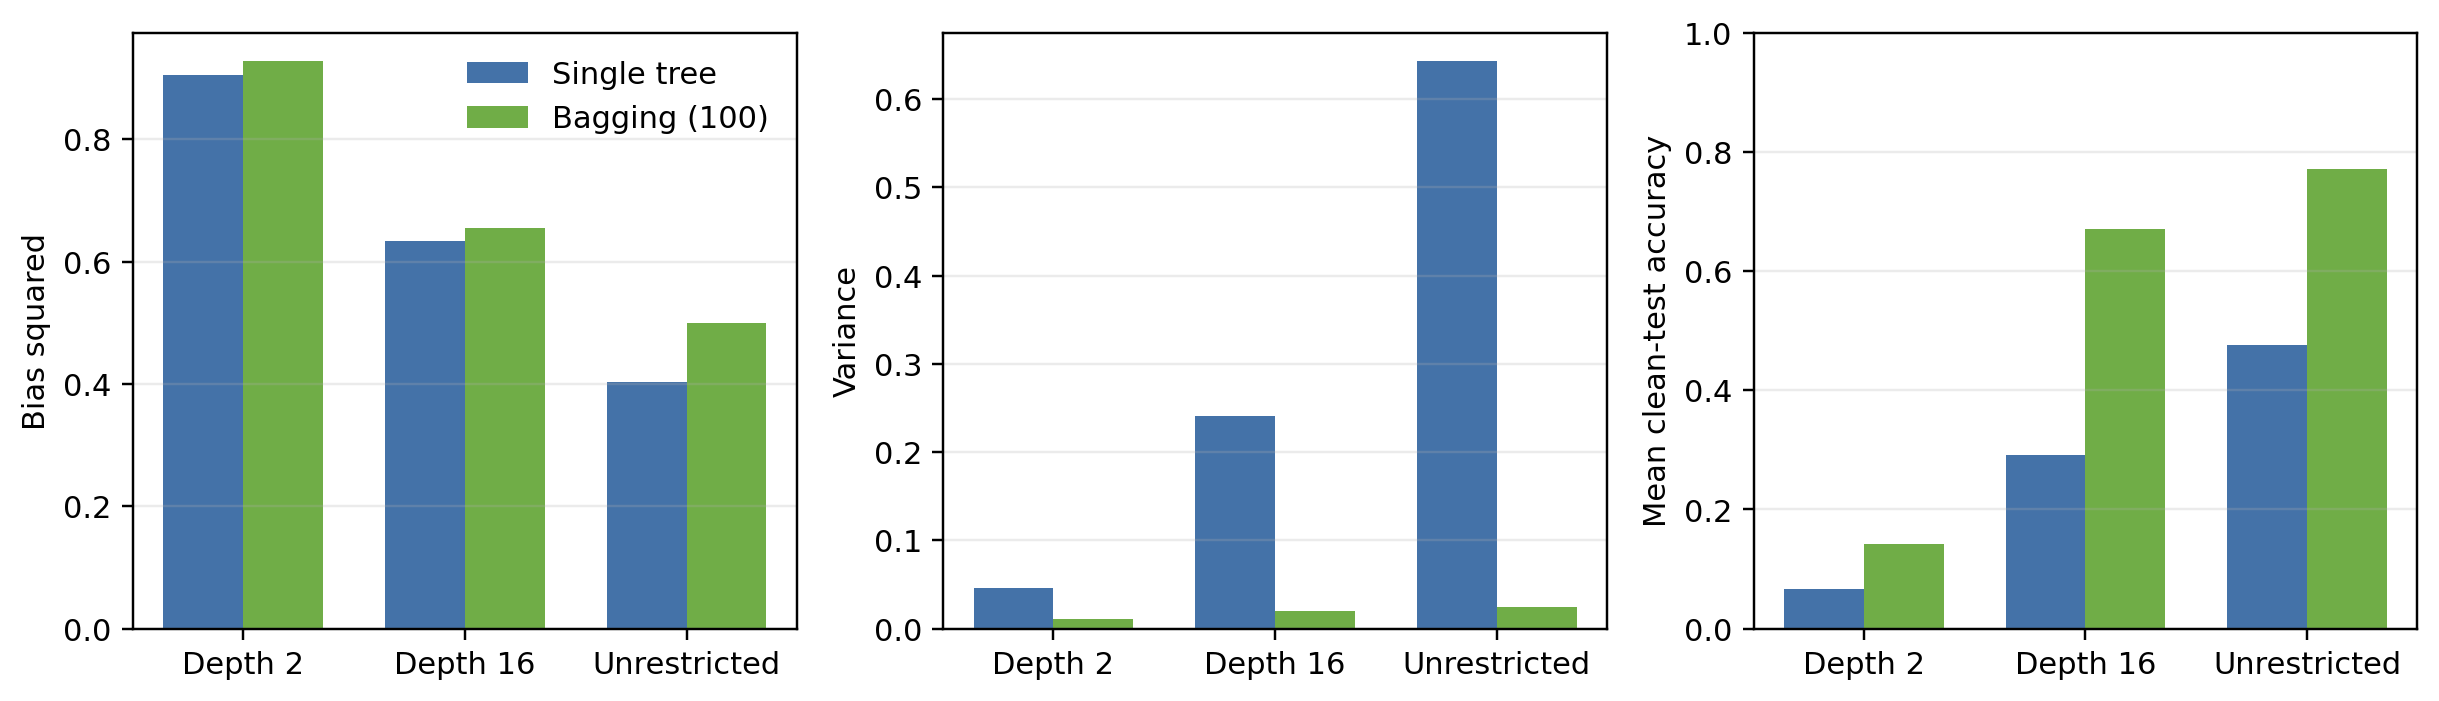
\includegraphics[width=0.94\textwidth]{../question_3/outputs/figures/q3b_depth_bias_variance_accuracy.png}
\caption{Bias$^2$, variance and mean clean-test accuracy across the three predeclared depth settings.}
\end{figure*}

\begin{figure*}[t]
\centering
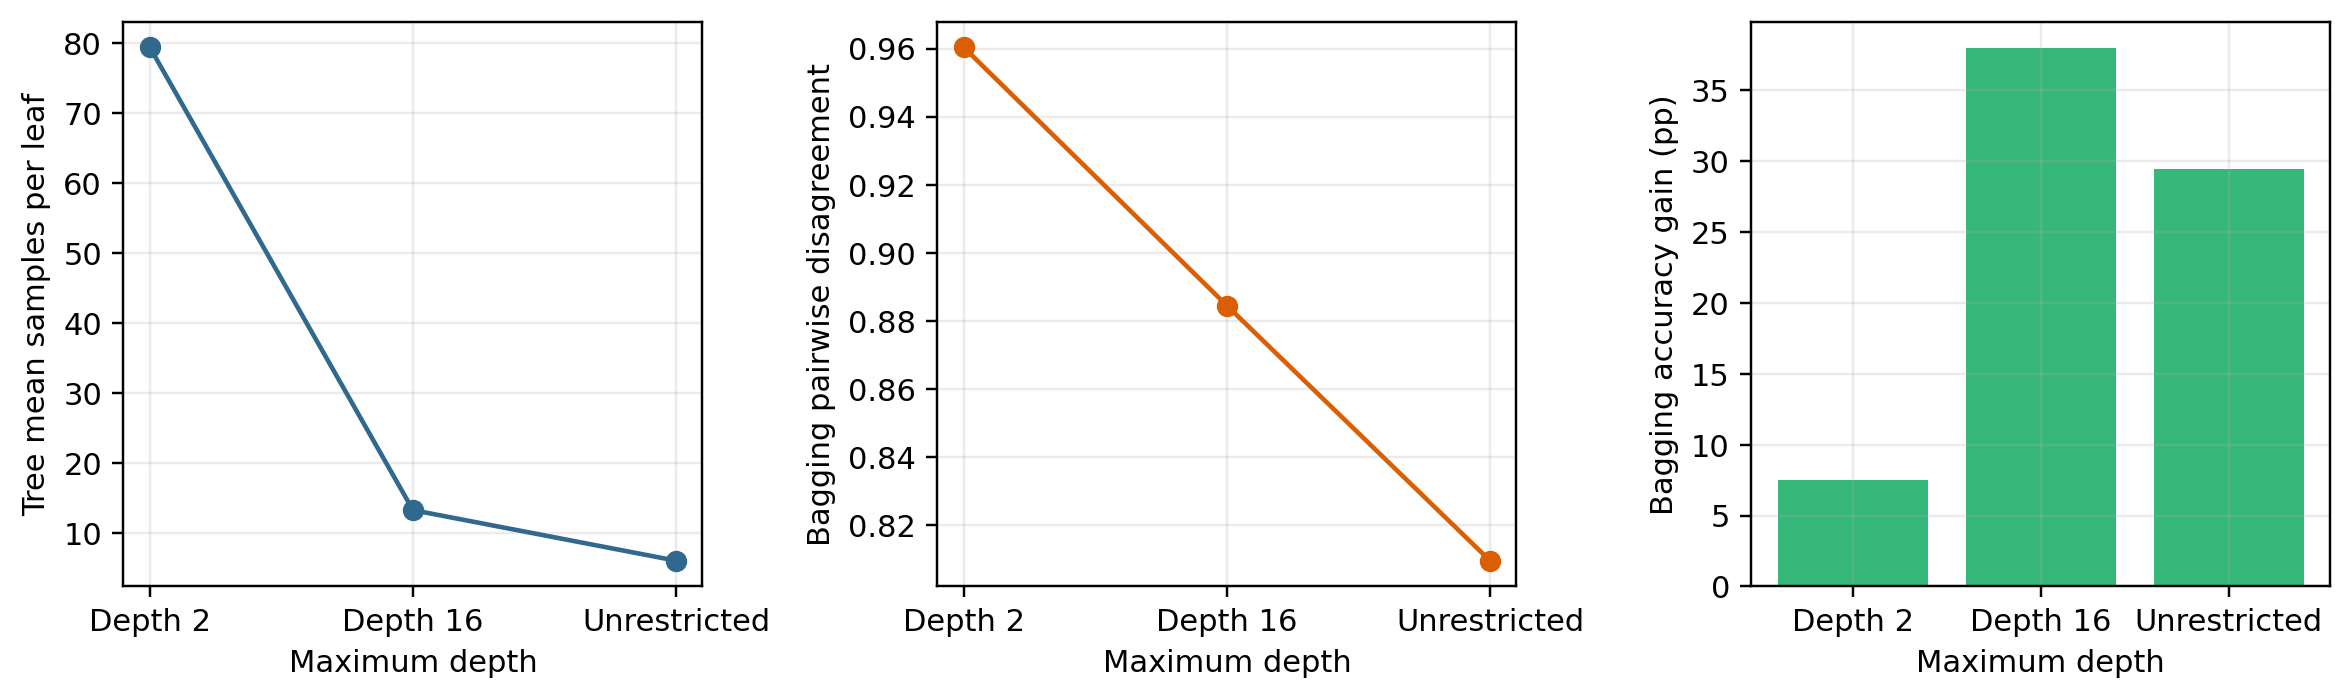
\includegraphics[width=0.94\textwidth]{../question_3/outputs/figures/q3c_depth_evidence.png}
\caption{Leaf occupancy, pairwise disagreement and the accuracy gain from 100-tree bagging.}
\end{figure*}

\textbf{No.} Bagging improves accuracy by 7.50 points at depth 2, 37.96 at depth 16, and 29.46 for unrestricted trees. The deepest trees show the largest variance reduction, but not the largest accuracy gain.

A depth-2 tree has 3.03 leaves and 79.33 training cases per leaf on average. Its bias is 0.90476. Disagreement is high (0.9604), but it represents diversity among crude, mostly wrong partitions; the bagged model reaches only 14.21\%.

At depth 16, a tree averages 18.27 leaves and 13.23 cases per leaf. Bias has fallen to 0.63420, while variance 0.24113 leaves enough instability to average away. Disagreement remains high at 0.8844, and bagging reaches 67.12\%. This balance produces the largest gain.

Unrestricted trees average depth 34.9, 40 leaves and six cases per leaf. Their lower bias (0.40394) and higher starting accuracy leave less headroom. Bagging removes 96.19\% of variance, but bias rises to 0.49893 and disagreement is lower at 0.8094. Variance removal and discrete accuracy improvement are therefore related but not interchangeable.

\subsection{Final accuracy and robustness summary}
\begin{table}[h]
\centering\scriptsize
\resizebox{\columnwidth}{!}{%
\begin{tabular}{lrrrrr}
\toprule
Model & Clean & Masked & $\Delta$ & Bias$^2$ & Variance \\
\midrule
Tree & 57.50 & 33.75 & $-23.75$ & 0.40394 & 0.64272 \\
Bagging & \textbf{87.50} & \textbf{70.00} & $-17.50$ & 0.49887 & 0.02062 \\
Boosting & 52.50 & 53.75 & $+1.25$ & 0.88015 & \textbf{0.01587} \\
\bottomrule
\end{tabular}}
\end{table}

The frozen tree is most sensitive to missing pixels and most sensitive to resampled training data. Bagging is the best recogniser on both test sets and remains stable across refits. Boosting has the lowest variance and smallest observed mask change, but also the highest bias. Its one-image masked gain accompanies lower winning confidence, so it is not evidence of genuine robustness.

\section{Discussion}
The experiments separate three ideas that can look similar in a single accuracy number. First, deep trees are expressive but unstable: their class vectors vary sharply when a few training faces are duplicated or omitted. Second, bagging works well here because these unstable trees make sufficiently different errors, and plurality voting preserves useful identity detail while removing much of the variability. Third, boosting's sequential focus is reproducible, but the depth-4 learners retain a strong systematic error on this 40-class task. Low variance cannot compensate for that bias.

\clearpage
\section{Reproducibility and checks}
The repository contains the saved split, roll-number seed, frozen JSON configurations, scratch bagging and boosting code, raw CSV tables, run logs, plotting code, figures and exact commands. Versions are pinned in \texttt{requirements.txt}. The official environment used Python 3.13.7, NumPy 2.2.6 and scikit-learn 1.7.2.

Three independent verification programs check selection rules, vector normalisation, OOB conventions, SAMME updates, saved case votes and the Q3 formulas. The Q3 verifier also checks all 30 resamples, eight arrays of shape $(30,80,40)$, per-repetition checkpoints and the identity-wise sampling rule. The complete unit-test suite contains 12 passing tests.

The 30-refit Q3 run used deterministic child seeds and took 1740.85 seconds with ten parallel jobs. Its resample digest begins \texttt{956e0203} and protocol digest begins \texttt{1de73ca9}. These identifiers prevent cached checkpoints from being mixed across protocols.

\section{Limitations}
All conclusions are conditional on one roll-number split and an 80-image test set. A 1.25-point accuracy change is one image, so small clean/masked differences should not be overinterpreted. Timing comparisons are specific to this machine and to the measured fitting boundary. Finally, the Q3 resampling distribution is centred on the six observed training faces per identity; it measures training-sample sensitivity within this assignment protocol, not population-wide facial variation.

\section{Conclusion}
On this split, the selected 200-tree bagged classifier gives the best balance of accuracy, stability and missing-region tolerance. Its clean accuracy is 30 points above the single tree and 35 points above selected boosting. Measured variance confirms that aggregation stabilises deep trees, while the depth study shows why the largest variance reduction need not produce the largest accuracy gain. Boosting supplies the counterexample needed for the final comparison: it has the lowest variance, yet high bias keeps its accuracy below bagging.

\begin{thebibliography}{9}
\small
\bibitem{samaria1994}
F. Samaria and A. Harter. Parameterisation of a stochastic model for human face identification. In \emph{Proc. 2nd IEEE Workshop on Applications of Computer Vision}, pages 138--142, 1994. doi:10.1109/ACV.1994.341300.

\bibitem{breiman1996}
L. Breiman. Bagging predictors. \emph{Machine Learning}, 24(2):123--140, 1996. doi:10.1007/BF00058655.

\bibitem{zhu2009}
J. Zhu, H. Zou, S. Rosset, and T. Hastie. Multi-class AdaBoost. \emph{Statistics and Its Interface}, 2(3):349--360, 2009. doi:10.4310/SII.2009.v2.n3.a8.

\bibitem{pedregosa2011}
F. Pedregosa et al. Scikit-learn: Machine learning in Python. \emph{Journal of Machine Learning Research}, 12(85):2825--2830, 2011.
\end{thebibliography}

\end{document}
